%\vspace{3cm}
\subsection{Polarized Target}
This experiment will require the installation of the
UVa polarized target operated in longitudinal and also transverse mode.  Transverse polarization requires  operation of an upstream chicane to ensure proper transport through the target magnetic field.  The target is typically operated with a specialized slow raster, and beamline instrumentation capable of characterizing the low current 50-100 nA beam.
All of these requirements have been met previously in Hall C, and will be soon implemented
also in Hall A for the E08-027/E08-007 run in 2011. 
%
The UVa polarized target (see Fig.~\ref{fig:target}), 
has been successfully used in experiments E143, E155, and E155x at SLAC, and E93-026, E01-006 and E07-003 at JLab. In 2011, the same target will be utilized in experiments E08-027 and E08-007. 
A similar target was used in Hall B for the EG1,EG4 and DVCS experiments, although Hall B does
not at present have the facilities necessary for transverse polarization.
%
\begin{figure}[h]
\centering
\includegraphics[width=2.5in,clip]{figs/target_gimp.eps}
\caption{Cross section view of the polarized target  \label{fig:target}}
\end{figure}

The UVa target operates on the principle of Dynamic Nuclear Polarization, to
enhance the low temperature (1 K), high magnetic field (5 T) polarization of solid
materials  by microwave pumping.
The polarized target assembly contains several target cells of 3.0 cm length
that can be  selected individually by remote control to be located in the uniform field
region of a superconducting Helmholtz pair. The permeable target cells are
immersed in a  vessel filled with liquid Helium and maintained at 1 K by use of a
high power evaporation refrigerator.
The coils have a 50$^\circ$ conical shaped aperture along the beam axis
which allow for unobstructed forward scattering.
%34$^\circ$ wedge shaped aperture along the vertically oriented midplane.

The target material is exposed to 140 GHz microwaves
to drive the hyperfine transition which  aligns the nucleon spins. 
 The heating of the target by the beam causes a drop of a few percent in
the polarization, and the polarization slowly decreases with time due to radiation
damage. Most of the radiation damage can be repaired by annealing the target at
about 80 K, until the accumulated dose reached is greater than about 
$ 17\times 10^{15}$ e$^-$/cm$^2$, at
which time the target material needs to be replaced. The luminosity of the polarized 
material in the uniform field region is approximately $85\times 10^{33}$ cm$^{-2}$ Hz.

\subsubsection*{Tensor Polarization}
When a  spin 1 system such as the deuteron is subjected to a magnetic field along the z-axis, the
Zeeman interaction gives rise to three magnetic sublevels $I_z = +1,0,-1$ with
population fractions $p_+,p_-, p_0$, respectively.
%\footnote{i.e. $p_+ + p_- +p_0=1$.}. 
These populations are described by
both a vector  polarization,
%
\begin{eqnarray}
\nonumber
P_z &=&\langle I_z/I\rangle \\ 
    &=&(p_+ - p_0) + (p_0-p_+) = p_+ - p_-
\end{eqnarray}
and a tensor polarization~\cite{Meyer:1985dta}:
\begin{eqnarray}
\nonumber
P_{zz} &=& \langle 3 I_z^2 - I(I+1)\rangle/I^2   \\
&=&(p_+ - p_0) - (p_0-p_-) = 1 - 3 p_0
\end{eqnarray}
%
which are subject to the overall normalization $p_+ + p_- + p_0 = 1$.
%
In the case of deuteron spins in thermal equilibrium with the solid lattice, and neglecting the small quadrupole interaction~\cite{Meyer:1985dta}, the tensor polarization is related to  the vector polarization via:
\begin{eqnarray}
P_{zz}= 2 - \sqrt{4-3 P_z^2}
\end{eqnarray}
This relation allows calculation of a target's tensor polarization once the vector polarization has been determined from standard NMR techniques. Vector polarizations can be determined by analyzing NMR lineshapes as described in~\cite{Dulya:1997qc} with a typical  7\% relative uncertainty, or by comparison of the NMR response to the known thermal equilibrium (TE) polarization.

The DNP technique produces  deuteron vector polarizations of up to 60\%  in ND$_3$ and 64\% in LiD~\cite{Bueltmann:1998wq}, which corresponds to tensor polarizations of approximately 30\%.
Tensor polarizations of 22\% have been achieved in previous experiments~\cite{Meyer:1985dta}
using standard solid polarized ammonia targets.
At the University of Virginia and the University of New Hampshire, 
we are pursuing techniques to enhance the tensor polarization by directly stimulating 
transitions to/from the $M_s=0$ state.  The UVa group  had some initial 
success in obtaining enhanced tensor polarizations via RF pumping, although the method was not pursued due to
lack of need for tensor polarized targets at the time of the study.  Another method entails simultaneously pumping 
the paramagnetic centers with two independent microwave frequencies, which requires careful isolation of the 
respective microwave cavities. As this work is on-going, the rates in this proposal assume only  tensor polarizations that have been demonstrated previously.



